% !TeX root = ./user_manual.tex
\documentclass[../../report.tex]{subfiles}

\begin{document}

\chapter{User manual: \texttt{recap} library}
\label{chap:user_man_recap}

\emph{Recap} is a tool for providing \emph{REproducible Configurations for Any Project}.
Research should be reproducible.
Especially in deep learning, it is important to keep track of hyperparameters and configurations used in experiments.
This package aims at making that easier.

\section{Installing}
\label{sec:recap_installation}
Before installing this package, ensure that Python version 3.6 or greater is installed on the host system.
Furthermore, ensure that the Python package installer \texttt{pip} is installed.

The preferred way of installing this package is to install it directly from \gls{pypi} by running the command:
\begin{minted}{bash}
pip install recap
\end{minted}

However, it is also possible to install it from source using the \emph{Poetry} tool for managing Python dependencies:
\begin{minted}{bash}
pip install poetry
cd recap
poetry install
poetry shell
\end{minted}
Poetry will automatically create a virtual Python environment for this project.
Running \mintinline{bash}|poetry shell| at the end opens a shell in the virtual environment. 
Ensure that this shell is used when running any of the other commands below.

Finally, to just install \texttt{recap} globally without using Poetry, one may instead run:
\begin{minted}{bash}
cd recap
pip install .
\end{minted}

\section{Usage}
Recap provides two top-level concepts that can be imported as follows:
\begin{minted}{python3}
from recap import URI, CfgNode as CN
\end{minted}

The \py{CfgNode} is a subclass of \py{CfgNode} from the \emph{yacs} package.
It provides some additional features for parsing configurations that are inherited between files which is not possible with yacs.

Recap's \py{URI} class provides a mechanism for handling logical paths within your project more conveniently with an interface that is fully compatible with \py{pathlib.Path}.

\subsection{\Acs{yaml} configurations}
Configurations are defined just like in yacs, except that the \py{CfgNode} class must be imported from the \texttt{recap} package instead of yacs.
Consider the following \gls{yaml} configuration that sets default values for all configuration options that will be used in the project.
A good name for this file is \texttt{\_base.yaml} because all experiments will build on these values.
\begin{minted}{yaml}
SYSTEM:
  NUM_GPUS: 4
  NUM_WORKERS: 2
TRAIN:
  LEARNING_RATE: 0.001
  BATCH_SIZE: 32
  SOME_OTHER_HYPERPARAMETER: 10
\end{minted}

The equivalent configuration can be obtained programatically like so:

\begin{minted}{python3}
from recap import CfgNode as CN

cfg = CN()
cfg.SYSTEM = CN()
cfg.SYSTEM.NUM_GPUS = 4
cfg.SYSTEM.NUM_WORKERS = 2
cfg.TRAIN = CN()
cfg.TRAIN.LEARNING_RATE = 1e-3
cfg.TRAIN.BATCH_SIZE = 32
cfg.TRAIN.SOME_OTHER_HYPERPARAMETER = 10
print(cfg)
\end{minted}

\subsubsection{Inheriting configurations}
Recap provides functionality for inheriting configuration options from other configuration files by setting the top-level \mintinline{yaml}{_BASE_} key.
So, one could create a configuration file \path{experiment_1.yaml} for an experiment with a different learning rate and batch size:

\begin{minted}{yaml}
_BASE_: _base.yaml

TRAIN:
  LEARNING_RATE: 1e-2
  BATCH_SIZE: 64
\end{minted}

In the code, to load the experiment configuration, one would use the function \py{recap.CfgNode.load_yaml_with_base()} like so:

\begin{minted}{python3}
from recap import CfgNode as CN

cfg = CN.load_yaml_with_base("experiment_1.yaml")
print(cfg)
\end{minted}
The above code will output:
\begin{minted}{yaml}
SYSTEM:
  NUM_GPUS: 4
  NUM_WORKERS: 2
TRAIN:
  LEARNING_RATE: 0.01
  BATCH_SIZE: 64
  SOME_OTHER_HYPERPARAMETER: 10
\end{minted}
Note that the \mintinline{yaml}{_BASE_} keys can be arbitrarily nested;
however, circular references are prohibited.

\subsection{Logical \acsp{uri} and the path manager}
\label{sec:recap_uris}
Recap includes a path manager for conveniently specifying paths to logical entities.
The path strings are set up like a \gls{uri} where the scheme (i.e.\ \texttt{http} in the path string \texttt{http://google.com}) refers to a logical entity.
Each such entity needs to be set up as a \py{PathTranslator} that can translate the logical \gls{uri} path to a physical path on the file system.

For example, one could set up a path translator for the data scheme to refer to the the path of a dataset on our file system located at \path{/path/to/dataset}.
Then, the recap \gls{uri} \path{data://train/abc.txt} would be translated to the local path \path{/path/to/dataset/train/abc.txt}.
The simplest way of setting that up is using the \py{register_translator} function (although more complex setups are possible with the \py{PathTranslator} class, allowing for example the download of files from the internet):
\begin{minted}{python3}
from recap.path_manager import register_translator
from pathlib import Path

register_translator("data", Path("/path/to/dataset"))
\end{minted}
Then, the \py{recap.URI} class can be used just like any \py{pathlib.Path} object:
\begin{minted}{python3}
from recap import URI

my_uri = URI("data://train/abc.txt")
# Here, str(my_uri) == "/path/to/dataset/train/abc.txt"

with my_uri.open("r") as f:
    print(f.read())
\end{minted}


\subsubsection{Logical \acsp{uri} in inherited configurations}
The \py{recap.URI} interface is fully compatible with nested configurations.
This means that recap \glspl{uri} can be used within the \mintinline{yaml}{_BASE_} field for inheriting configurations.
For example, one could register a path translator for the config scheme and then include \mintinline{yaml}{_BASE_: config://_base.yaml} in the configuration files.

\section{Automated tests}
\label{sec:recap_tests}
To run the automated tests, run the following command from within the \texttt{recap} repository:
\begin{minted}{bash}
python -m pytest
\end{minted}
Note that this will not work if the \texttt{recap} package was installed directly via \texttt{pip} because that will not copy over the \texttt{tests} folder.
Instead, use one of the other two installation options given in \cref{sec:recap_installation}
Ensure that \texttt{poetry shell} is run before executing this command if the package was installed via Poetry.
A screenshot of the output is provided in \cref{lst:tests_recap}.

\section{Documentation}
\label{sec:recap_documentation}
More detailed documentation than this user manual is available at \url{https://recap.readthedocs.io}.
The package documentation includes detailed explanations of each of the submodules, methods, and classes.
The same documentation is provided in \gls{html} format alongside this submission at \path{docs/recap/index.html}.

\chapter{User manual: \texttt{chesscog} package}
\label{chap:user_man_chesscog}

\emph{Chesscog} combines traditional computer vision techniques with deep learning to identify chess positions from photos.
This repository contains all the code required to execute the chess recognition pipeline end-to-end as well as to train and fine-tune the \glspl{cnn} for unseen chess sets.
Furthermore, the evaluation scripts for the experiments conducted for this report are available in this package.

\section{Installing}
\label{sec:chesscog_installing}
Before installing this package, ensure that Python version 3.7 or greater is installed on the host machine.
Furthermore, ensure that the Python package installer \texttt{pip} is installed.
Then, navigate to the \texttt{chesscog} folder in the submission, or run \mintinline{bash}{git clone https://github.com/georgw777/chesscog.git}.

The easiest way to install the \texttt{chesscog} package and its dependencies is to run:
\begin{minted}{bash}
pip install .
\end{minted}

However, if desired, it may alternatively be installed using the \emph{Poetry} tool for managing Python dependencies.
To do so, first ensure that Poetry is installed by running \mintinline{bash}{pip install poetry} and then run:
\begin{minted}{bash}
cd chesscog
poetry install
poetry shell
\end{minted}
Poetry will automatically create a virtual Python environment for this project.
Running \mintinline{bash}|poetry shell| at the end opens a shell in the virtual environment. 
Ensure that this shell is used when running any of the other commands below.

\section{Usage}

As explained in \cref{sec:chesscog_implementation}, many Python files simultaneously act as scripts.
The following subsections provide instructions for running these scripts in order to carry out the main tasks of the chess recognition system.
The scripts themselves are explained in more detail in the documentation (see \cref{sec:chesscog_documentation}), but are also self-documenting when supplied with the \texttt{--help} command line option.

\subsection{Dataset}
\label{sec:user_man_chesscog_dataset}

The recommended method of obtaining the rendered dataset is by following the instructions in \cref{sec:user_man_chesscog_download_dataset} to download it.
However, for the sake of completeness, the following subsection details how the script used to generate the dataset was executed.

\subsubsection{Data synthesis}
To synthesise the 3D dataset, first install Blender. 
Then, the \texttt{chess} library must be installed in Blender's own Python interpreter.
On a Mac, this can be achieved by running:
\begin{minted}{bash}
cd /Applications/Blender.app/Contents/Resources/2.90/python/bin
./python3.7m -m ensurepip
./python3.7m -m pip install --upgrade pip
./python3.7m -m pip install chess
\end{minted}

Finally, from back in the \texttt{chesscog} directory, the data can be synthesised using the following command:
\begin{minted}{bash}
blender chess_model.blend --background --python scripts/synthesize_data.py
\end{minted}
Note that this requires the \texttt{chess\_model.blend} file, i.e.\ the 3D chess model as a Blender file.
However, this model is not supplied with the project submission due to its large file size.

\subsubsection{Downloading and splitting the dataset}
\label{sec:user_man_chesscog_download_dataset}
To download the dataset and then perform the train/val/test split, run the two following commands:
\begin{minted}{bash}
python -m chesscog.data_synthesis.download_dataset
python -m chesscog.data_synthesis.split_dataset
\end{minted}
The dataset will be downloaded to the \path{data://render} folder which by default maps to \path{~/chess_data} (the mapping is achieved using \texttt{recap}'s \acs{uri} interface detailed in \cref{sec:recap_uris}).
This directory contains three subfolders, \texttt{train}, \texttt{val}, and \texttt{test}.

\subsubsection{Format of the dataset}
In each of the three subfolders, the images are supplied in PNG format.
For every image file, there is a \gls{json} file with the same name (but \texttt{*.json} extension) that contains the associated labels.
The contents of that \gls{json} file is shown in \cref{lst:json_labels} for the running example in \cref{chap:data_synthesis}.
\begin{listing}
    \inputminted{json}{\subfix{../../data/3828.json}}
    \caption[Structure of the \acs{json} annotations generated for the running example image from \cref{chap:data_synthesis}.]{Structure of the \acs{json} annotations generated for the running example image from \cref{chap:data_synthesis} (see \cref{fig:data_synthesis_visualisation}).}
    \label{lst:json_labels}
\end{listing}
The training of the chess recognition system relies only on the \texttt{fen}, \texttt{white\_turn}, and \texttt{corners} fields which respectively provide the \gls{fen} description of the chess position on the board, the colour of the current player (indicating from which player's perspective the photo was taken), and the pixel coordinates of the chessboard's four corner points.
The origin of the coordinate system is the top left of the image.

Nonetheless, the \gls{json} file also contains information about the positions and rotations of the lights and camera in the 3D world coordinate system as explained in \cref{sec:3d_renders}.
Furthermore, the bounding boxes for each of the pieces on the board are supplied in the \texttt{pieces} field in the \gls{json} file.
The coordinates are supplied in the order $x_1,y_1,x_2,y_2$.
This information is useful for potential further research exploring the use of object detection models for chess recognition.

\subsection{Board localisation}
Code related to board localisation is in the \py{chesscog.corner_detection} module.
More specifically, the \py{chesscog.corner_detection.detect_corners} submodule contains the \py{find_corners()} method that takes as input an image (as a \py{numpy} array) and outputs the detected corner points.
This submodule simultaneously acts as a script that can be run as follows:
\begin{minted}{bash}
python -m chesscog.corner_detection.detect_corners img.png
\end{minted}
Here, \texttt{img.png} is to be replaced with the path to the input image.
\Cref{fig:example_detect_corners} shows the output of that script when supplied with the path \path{data://render/train/3828.png} which is the running example from \cref{chap:data_synthesis}.
\begin{figure}
    \centering
    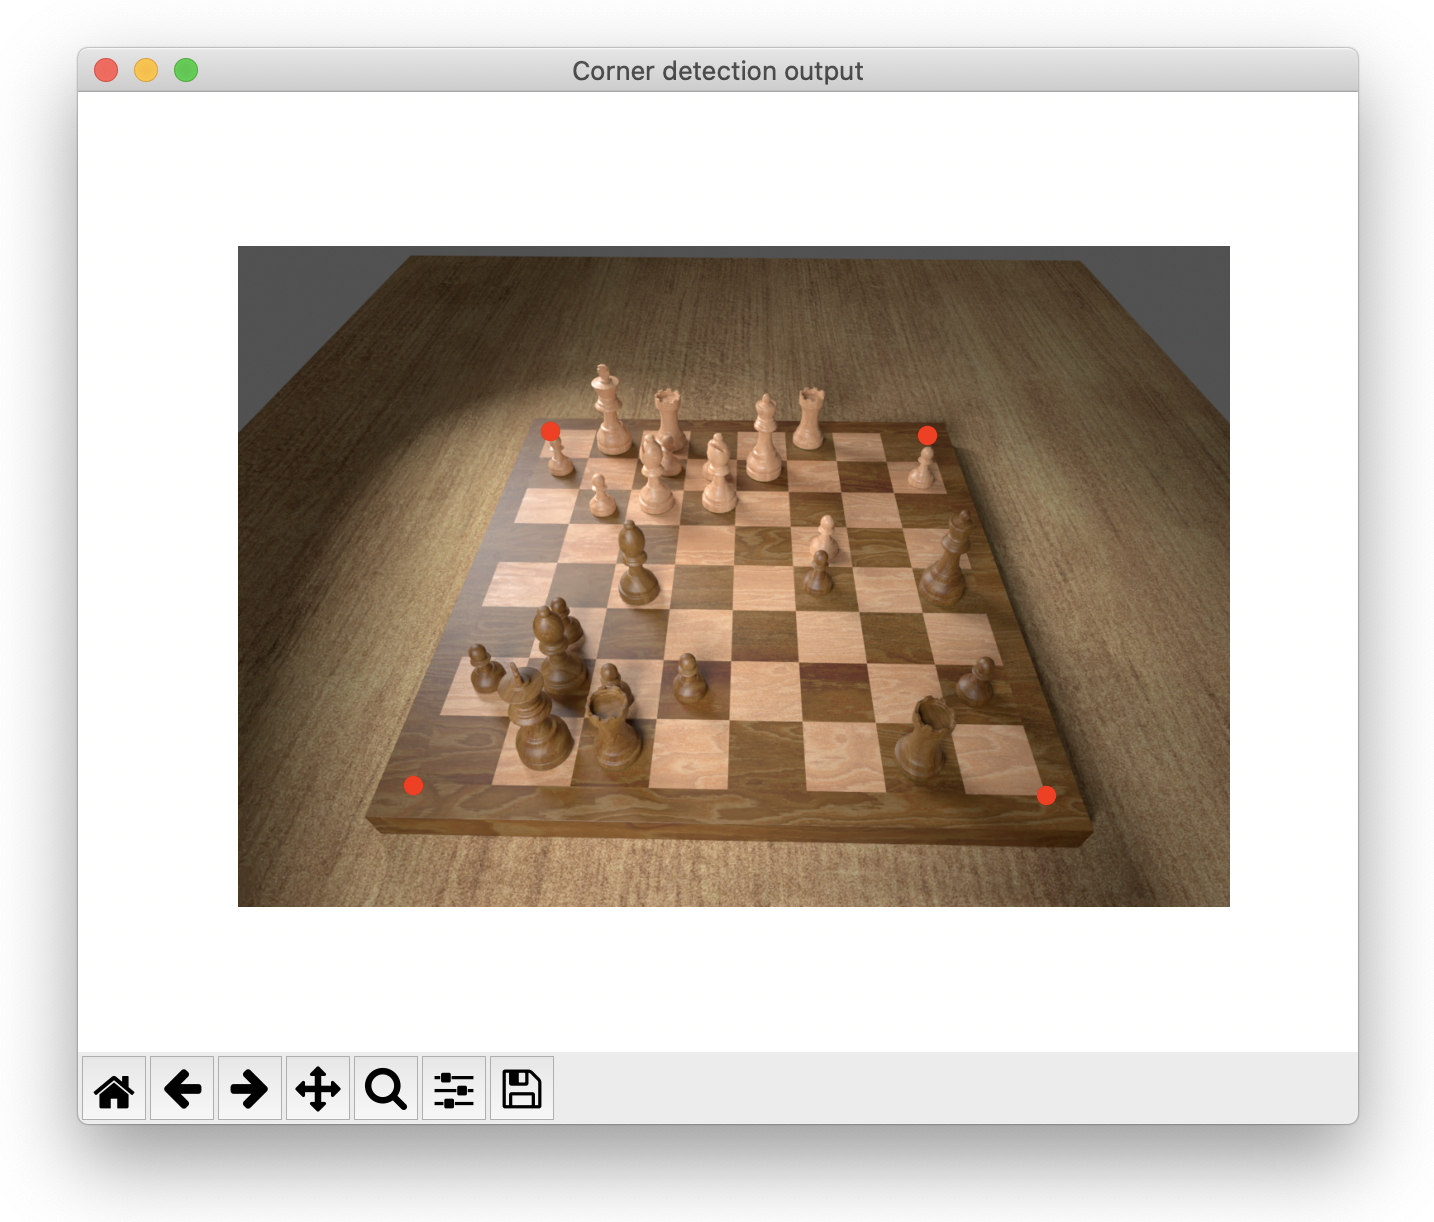
\includegraphics[width=.8\textwidth]{3828_corner_detection_screenshot}
    \caption{Screenshot of the corner detection output.}
    \label{fig:example_detect_corners}
\end{figure}

\subsection{Occupancy and piece classification}
Code for training and evaluating the occupancy and piece classifiers is located in the \py{chesscog.occupancy_classifier} and \py{chesscog.piece_classifier} modules respectively.
\subsubsection{Downloading the trained models}
\label{sec:chesscog_user_man_download_models}
To download the trained models, simply run:
\begin{minted}{bash}
python -m chesscog.occupancy_classifier.download_model
python -m chesscog.piece_classifier.download_model
\end{minted}
The models are downloaded to the \path{models://occupancy_classifier} and \path{models://piece_classifier} folders.
To find out where that is on the local file system, run the following Python snippet:
\begin{minted}{python3}
import recap
import chesscog # must be imported to properly configure recap
print(recap.URI("models://"))
\end{minted}
\subsubsection{Training the models}
\label{sec:chesscog_user_man_train}
To train the models yourself instead of using the already trained models (see previous section), the relevant datasets of the cropped squares must first be created by running:
\begin{minted}{bash}
python -m chesscog.occupancy_classifier.create_dataset
python -m chesscog.piece_classifier.create_dataset
\end{minted}
Then, the models can be trained by running:
\begin{minted}{bash}
python -m chesscog.occupancy_classifier.train
python -m chesscog.piece_classifier.train
\end{minted}
This will train all models specified using \gls{yaml} configuration files in the \path{config://occupancy_classifier} and \path{config://piece_classifier} folders.
It is recommended to use a machine with a CUDA-compatible \gls{gpu} for training.
To inspect the progress, run in a separate shell:
\begin{minted}{bash}
tensorboard --logdir ./runs
\end{minted}
The TensorBoard tool plots the key metrics live during training.
It should already be installed as per the instructions in \cref{sec:chesscog_installing}.
Finally, copy the folder of your selected piece and occupancy classifiers from \path{./runs} into \path{models://} so that these models will be used for inference and evaluation.

\subsection{Performing an inference}
\label{sec:chesscog_user_man_perform_inference}
The \py{chesscog.recognition} module is responsible for running the chess recognition pipeline end to end.
Further, the \py{chesscog.recognition.recognition} submodule provides the \py{ChessRecognizer} class that upon initialisation will load the \glspl{cnn} into memory and exposes the \py{predict()} method that when supplied with an input image will return the predicted \gls{fen} description.
This submodule also acts as a script that can be executed as follows:
\begin{minted}{bash}
python -m chesscog.recognition.recognition img.png --white
\end{minted}
Again, \texttt{img.png} should be replaced by the path to the desired input image (which may be a \texttt{recap} \gls{uri}).
The \texttt{--white} flag specifies the current player's perspective and can be replaced with \texttt{--black} for the other player.
\Cref{lst:chesscog_recognition_output} shows the output of that script.
\begin{listing}
    \verbatiminput{data/recognition_output.txt}
    \caption[Output of the chess recognition script.]{Output of the chess recognition script. Additional line breaks are added to fit on the page and are indicated with a backslash. White pieces are represented by uppercase letters while black pieces are denoted using lowercase letters.}
    \label{lst:chesscog_recognition_output}
\end{listing}
It provides the user with a text-based representation of the predicted chess position and a link to the chess engine analysis tool on the popular chess website \emph{Lichess} with that position set up.

\subsection{Performance evaluation}
\label{sec:chesscog_user_man_evaluate}
For evaluating the performance of the entire chess recognition pipeline on the test set, run:
\begin{minted}{text}
python -m chesscog.recognition.evaluate --save-fens --dataset test
\end{minted}
This creates a \gls{csv} file at \path{results://recognition/test.csv} that contains the prediction result (as well as other information like the number of mistakes) for each sample in the test set.
To obtain an overview of useful metrics (those shown in \cref{tbl:chess_recognition_trainvaltest_results}), run:
\begin{minted}{text}
python -m chesscog.report.prepare_recognition_results \
  --results results://recognition --dataset test
\end{minted}

The \py{chesscog.corner_detection}, \py{chesscog.occupancy_classifier}, and \py{chesscog.piece_classifier} modules each contain an \texttt{evaluate} submodule that acts in a similar manner to that of the whole system described above.
These modules facilitate the separate performance evaluation of the individual components of the pipeline.
For more information, run these scripts with the \texttt{--help} flag.

\subsection{Adapting to an unseen chess set}
To adapt the pipeline to an unseen chess set, first take a picture of the starting position from both players' perspectives, as illustrated in \cref{fig:transfer_learning_train_data}.
These two pictures constitute the \emph{training data} used to fine-tune the networks.
Name these two pictures \path{white.png} and \path{black.png} and place them in the \path{data://transfer_learning/images/train} folder.
Ensure that the two associated \gls{json} files (\texttt{white.json} and \texttt{black.json}) are exactly as indicated in \cref{fig:transfer_learning_json}.
\begin{listing}
    \begin{sublisting}[b]{\textwidth}
        \inputminted{json}{\subfix{../../data/transfer_learning/white.json}}
        \caption{white player's perspective}
    \end{sublisting}
    \medskip\par
    \begin{sublisting}[b]{\textwidth}
        \inputminted{json}{\subfix{../../data/transfer_learning/black.json}}
        \caption{black player's perspective}
    \end{sublisting}
    \caption{\Acs{json} labels of the two training images for the transfer learning task.}
    \label{fig:transfer_learning_json}
\end{listing}
Notice that these \gls{json} files simply contain the \gls{fen} string of the starting position (thus both are identical), as well as the boolean flag indicating the player's perspective.
This is all the information necessary to fine-tune the model!

Alternatively, the transfer learning dataset used in \cref{chap:adapting} can be downloaded by executing:
\begin{minted}{text}
python -m chesscog.transfer_learning.download_dataset
\end{minted}

\subsubsection{Fine-tuning the models}
The next step is to fine-tune the \glspl{cnn}. 
Ensure that the occupancy and piece classifiers trained on the rendered dataset are located in \path{models://occupancy_classifier} and \path{models://piece_classifier} as explained previously in \cref{sec:chesscog_user_man_train}.
Then, these models can be fine-tuned to the new dataset by running:
\begin{minted}{text}
python -m chesscog.transfer_learning.train
\end{minted}
This script first trains the occupancy classifier and then the piece classifier.
Both resulting models are then located in the \path{runs://transfer_learning} folder.
As explained in \cref{sec:chesscog_user_man_train}, the TensorBoard tool can be run concurrently in a different shell to inspect progress:
\begin{minted}{bash}
tensorboard --logdir ./runs
\end{minted}
Finally, if the results are satisfactory, copy over the models from \path{runs://transfer_learning} to \path{models://transfer_learning}.

Alternatively, the fine-tuned models from \cref{chap:adapting} can automatically be downloaded into the \path{models://transfer_learning} using the command:
\begin{minted}{bash}
python -m chesscog.transfer_learning.download_models
\end{minted}

\subsubsection{Performing an inference}
To perform an inference using the fine-tuned models, the same command line interface as in \cref{sec:chesscog_user_man_perform_inference} is implemented for the adapted pipeline.
Simply run the following command, substituting as indicated in \cref{sec:chesscog_user_man_perform_inference}:
\begin{minted}{bash}
python -m chesscog.transfer_learning.recognition img.png --white
\end{minted}

\subsubsection{Evaluating the fine-tuned pipeline}
To evaluate the pipeline, create a labelled test dataset in \path{data://transfer_learning/images/test}.
Then, use the \py{chesscog.transfer_learning.evaluate} module to evaluate the performance of the pipeline in the same way as explained in \cref{sec:chesscog_user_man_evaluate}.

\section{Automated tests}
\label{sec:chesscog_tests}
To run the automated tests, run the following command from within the \texttt{chesscog} repository:
\begin{minted}{bash}
python -m pytest
\end{minted}
Ensure that \texttt{poetry shell} is run before executing this command if the package was installed via Poetry.
A screenshot of the output is provided in \cref{lst:tests_chesscog}.

\section{Documentation}
\label{sec:chesscog_documentation}
More detailed documentation than this user manual is available at \url{https://georgw777.github.io/chesscog}.
The package documentation includes detailed explanations of each of the submodules, methods, and classes.
The same documentation is provided in \gls{html} format alongside this submission at \path{docs/chesscog/index.html}.

\chapter{User manual: web app}
\label{chap:user_man_chesscogapp}

The web app provides a proof of concept to demonstrate the functionality of the chess recognition pipeline.

\section{Installing}
The web app can be accessed at \url{https://www.chesscog.com} without any installation.
However, one may instead wish to run the web app locally using the installation instructions below.
Sometimes the inference system at the above mentioned URL encounters issues due to the memory limitations imposed by the free hosting plan, a problem explained in \cref{chap:implementation}.
In that case, running the web app locally is the best option.

First, ensure that Docker Compose is installed on the host system.
Then, from within the \texttt{chesscog-app} directory, simply run
\begin{minted}{bash}
docker-compose -f docker-compose.prod.yml up --build
\end{minted}
This command starts two Docker containers (the frontend and the backend).
In building the backend \gls{api}, the trained models will automatically be downloaded to the container as per the instructions from \cref{sec:chesscog_user_man_download_models}.
To open the web app, navigate to \url{http://localhost:80}.

\section{Usage}
Upon opening the web app in a browser (using either method described above), the landing page appears (see \cref{fig:chesscogapp_landing_page}).
\begin{figure}
    \centering
    \begin{subfigure}[b]{\textwidth}
        
\includegraphics[width=\textwidth]{screenshot_chesscogapp_landing_page}
        \caption{landing page}
        \label{fig:chesscogapp_landing_page}
    \end{subfigure}
    \hfill
    \medskip\par
    \begin{subfigure}[b]{\textwidth}
        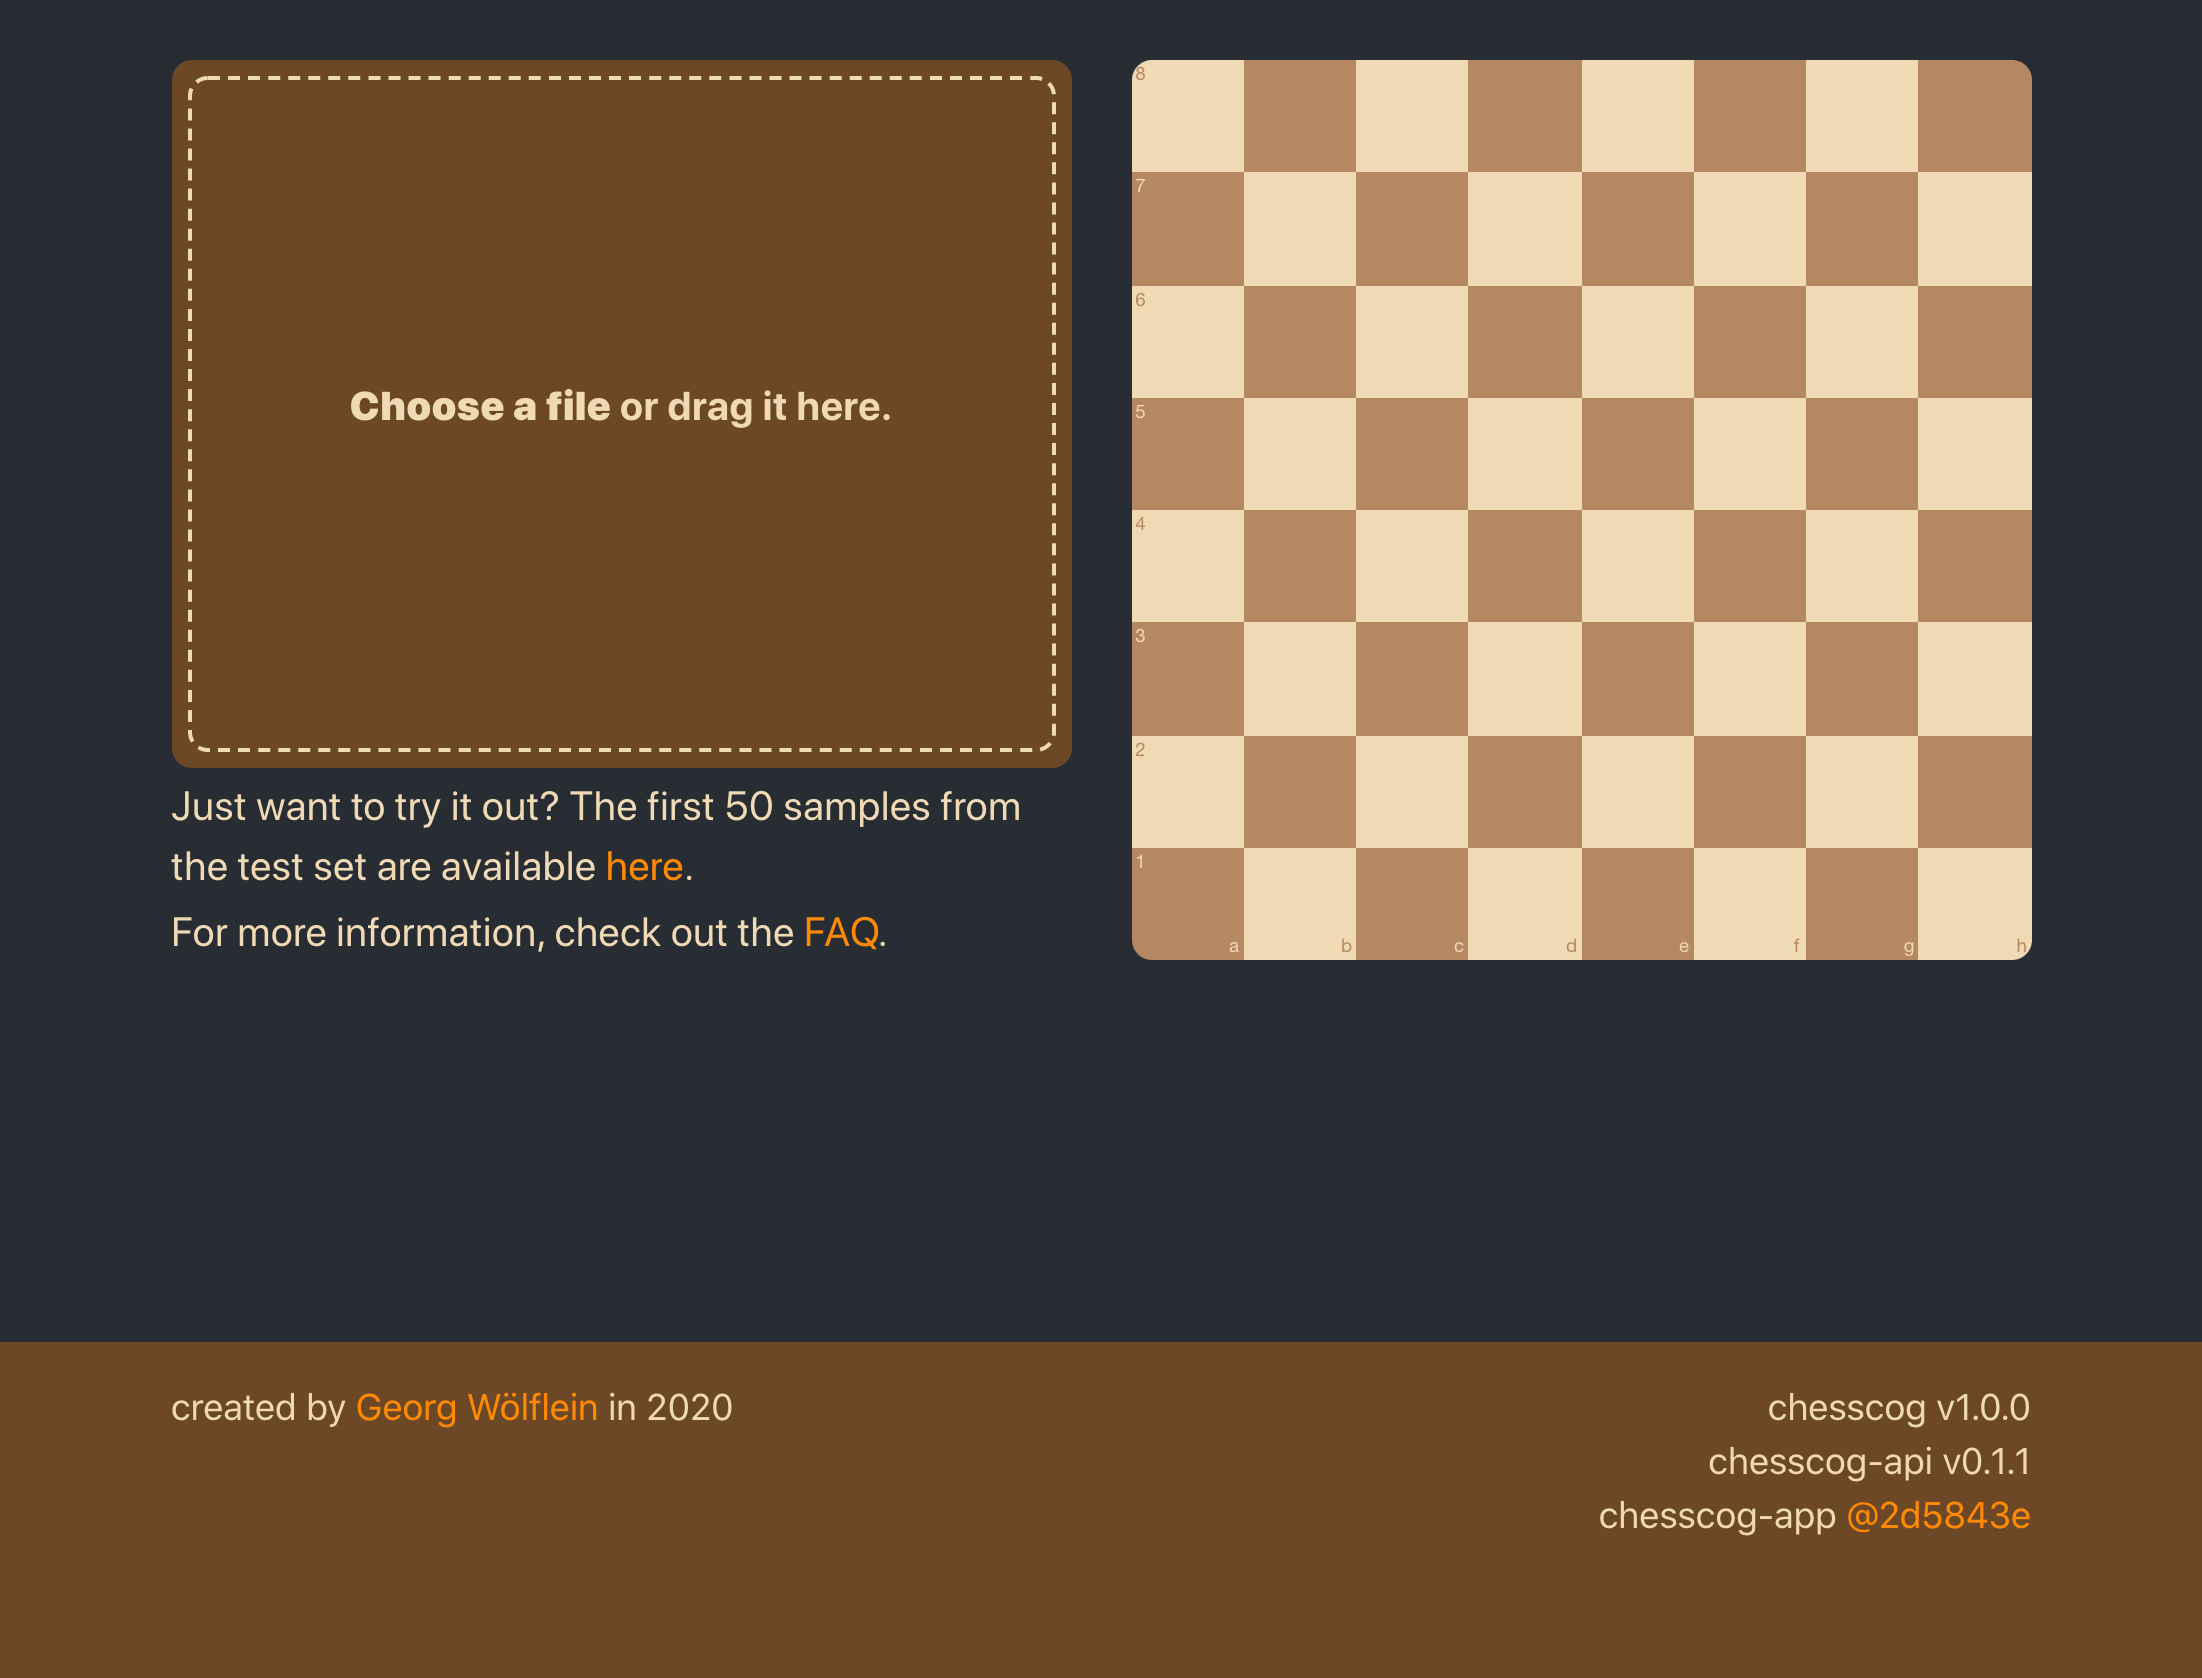
\includegraphics[width=\textwidth]{screenshot_chesscogapp_app}
        \caption{main app}
        \label{fig:chesscogapp_main_app}
    \end{subfigure}
    \caption{Screenshots of the web app.}
\end{figure}
Simply click the ``try it out'' button and the web page will scroll down to the main app depicted in \cref{fig:chesscogapp_main_app}.
Either drag and drop a photo of a chessboard onto the left-hand panel, or click on the panel to upon a file upload prompt.
Upon uploading the file, a preview is displayed, and a button labelled ``go'' appears.
Select either ``white to play'' or ``black to play'' and then click on that button to start the inference (a loading animation is shown on the chessboard while the chess recognition pipeline is processing the image).
Once the inference completes, the web app looks as depicted in \cref{fig:chesscogapp_inference} and displays the predicted position on the right.
Click the button on the right of the ``go'' button with the Lichess symbol in order to open that position on the popular chess website Lichess.
Finally, to perform another inference, click the ``reset'' button.

\section{Automated tests}
\label{sec:chesscogapp_tests}
There are automated tests for the frontend app written in TypeScript and the backend \gls{api} written in Python.
To run these tests, the relevant dependencies must first be installed, so ensure that the host system has the Poetry tool for managing Python dependencies as well as the Node package manager \texttt{npm}.
The following script installs the necessary dependencies and runs the tests for the backend and frontend.
Ensure that the current working directory is the root of the \texttt{chesscog-app} repository before executing the following commands.
\begin{minted}{bash}
# Backend tests
cd api
poetry install
poetry run python -m pytest
# Frontend tests
cd ../app
npm install
npm test
\end{minted}
\Cref{lst:tests_chesscogapp} shows the outputs of the automated tests for both components (frontend and backend).

\section{Documentation}
The web app is documented by way of a user-centric ``frequently asked questions'' page that addresses common issues and questions.
This page can be accessed at \url{https://www.chesscog.com/faq} and \cref{fig:chesscogapp_faq} shows a screenshot.
\begin{figure}
    \centering
    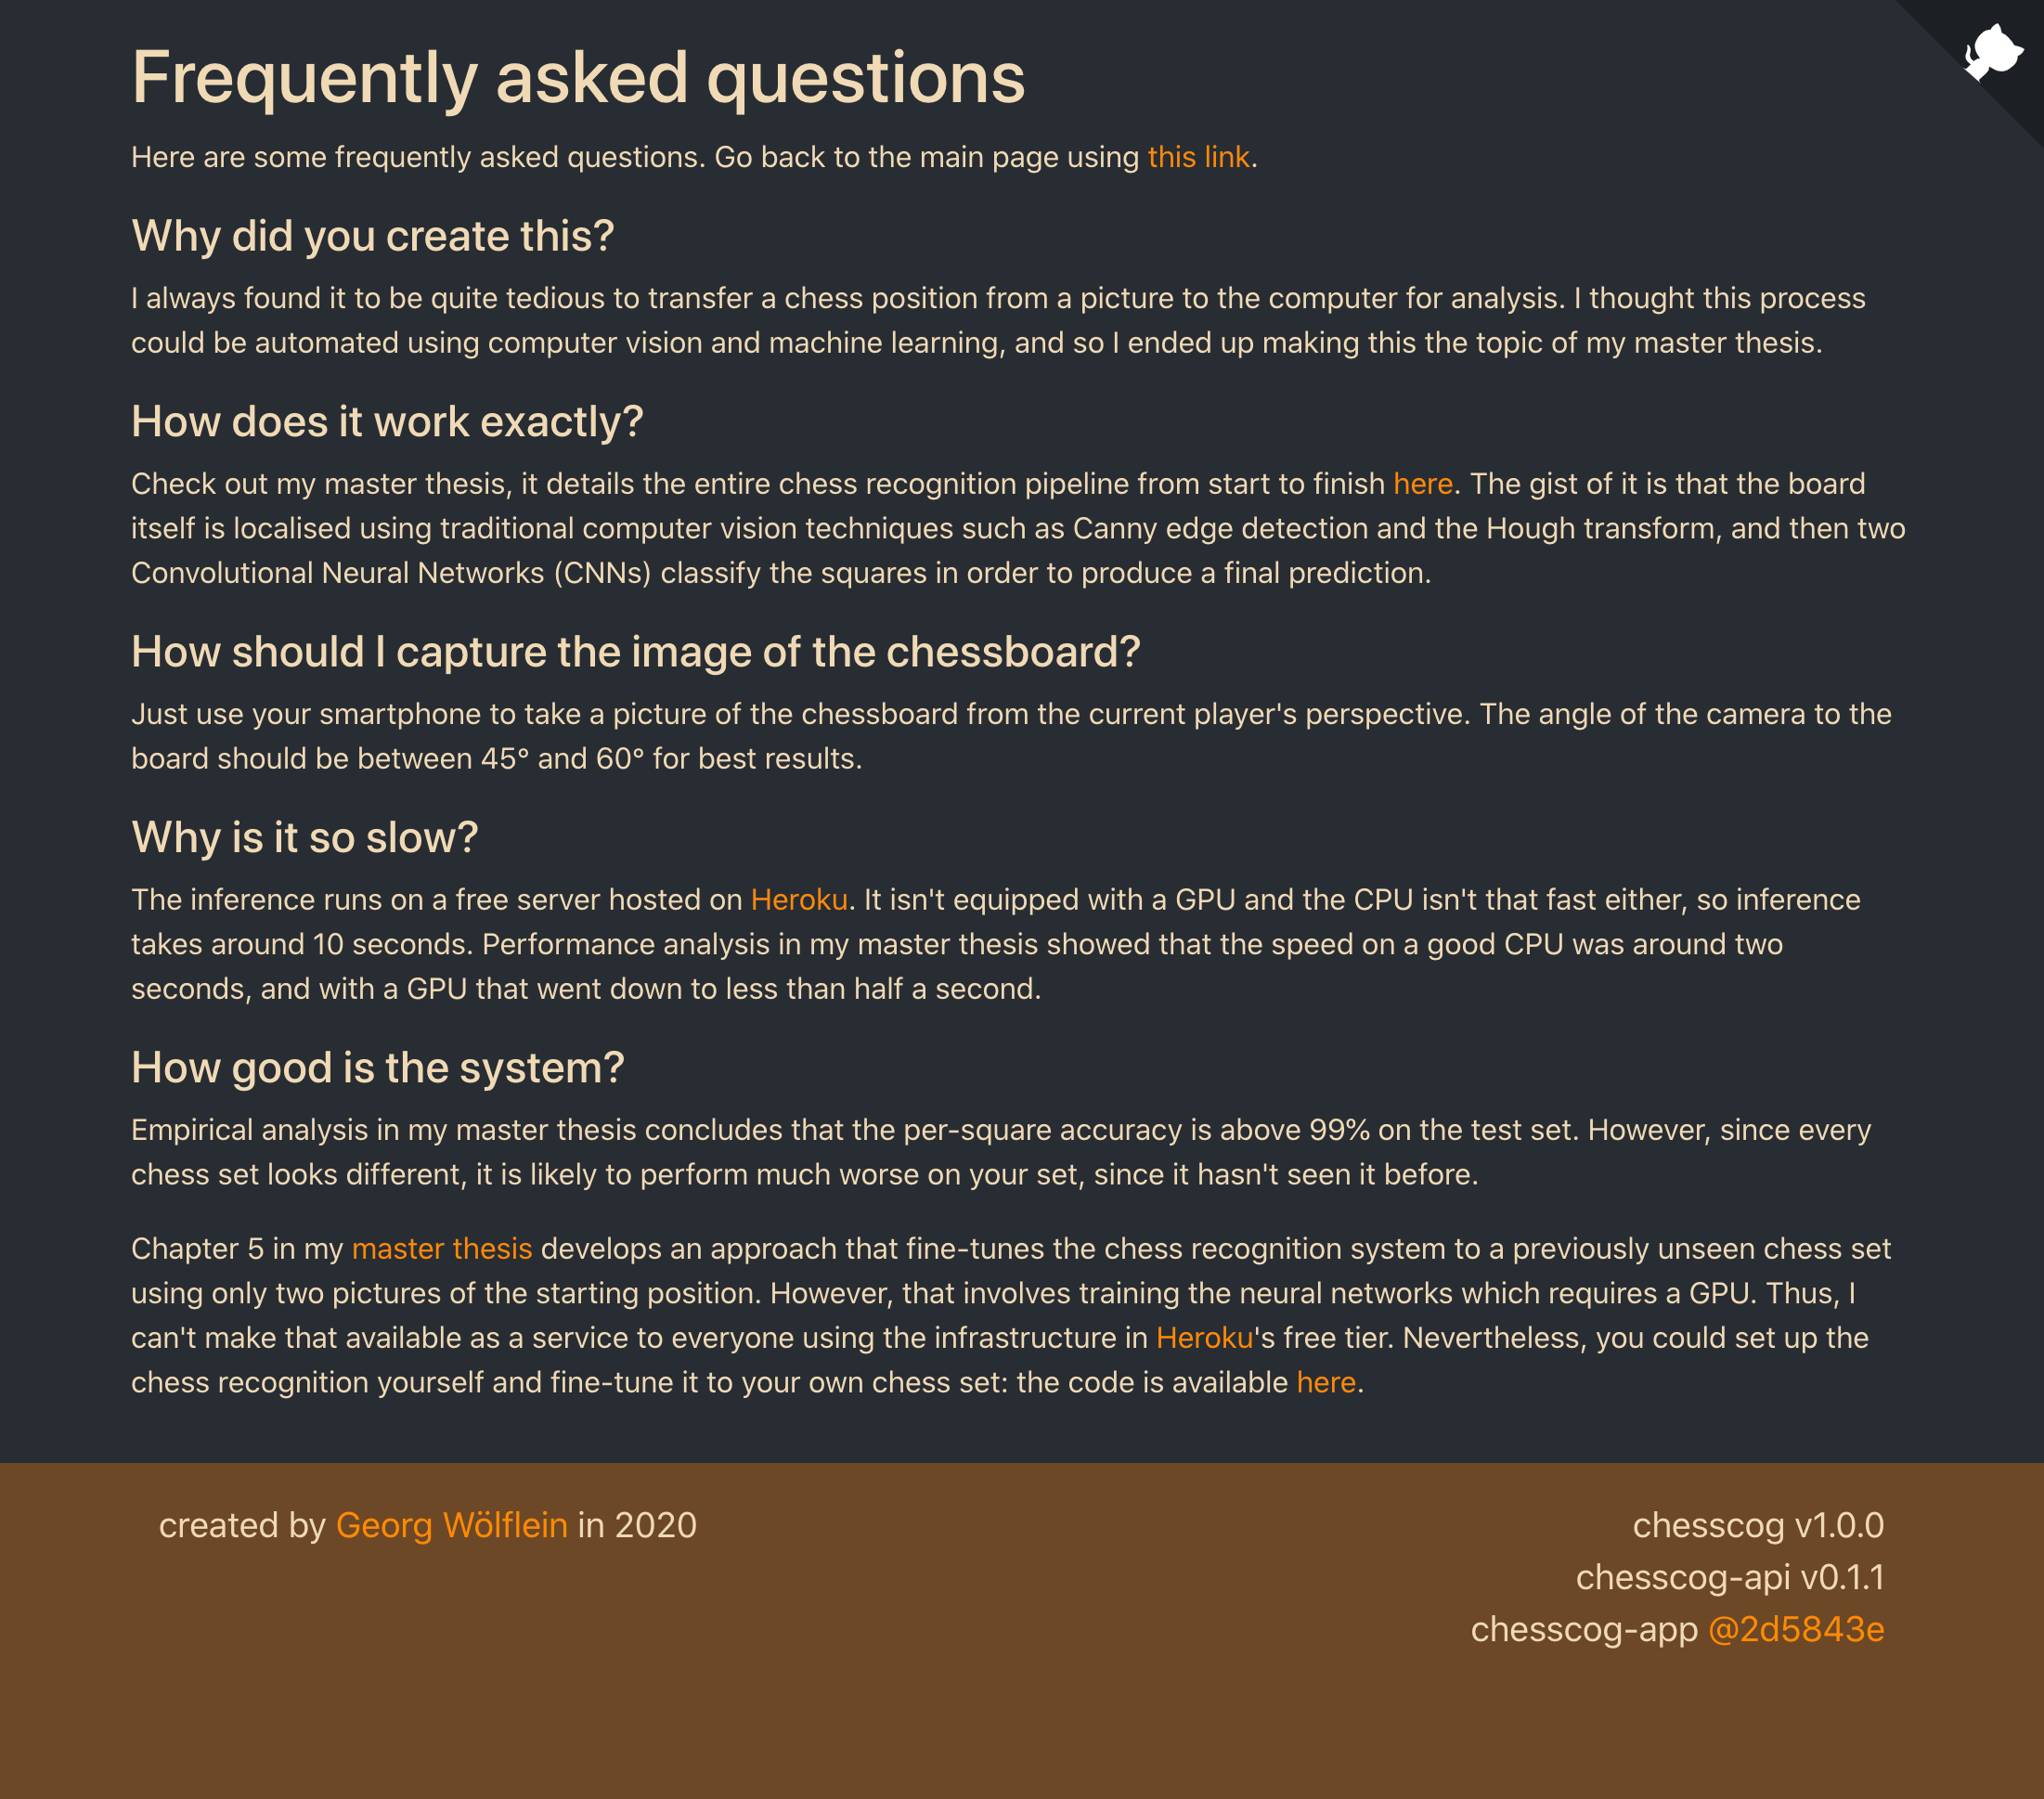
\includegraphics[width=\textwidth]{screenshot_chesscogapp_faq}
    \caption{Screenshot of the frequently asked questions page.}
    \label{fig:chesscogapp_faq}
\end{figure}


\end{document}